% !TeX spellcheck = en_US
\chapter{Coding Languages And Tools}

Across the time working on the thesis and the internship, I had the opportunity to experience the professional workflow with state-of-the-art methods. This section summarizes common languages, tools for developers and the workflow. In addition the presented languages and tools, I also either worked with or got to know more about Docker \cite{merkel2014docker}, Python, Vim, git, \etc.

\section{Bash}

\subsection{Introduction}

Linux is a family of operating systems based on the Linux kernel. For public users, it is less common and well-known comparing to Windows and Mac. These two receive more attention for application developments, however, give little access to the source code and are more prone to malware. On the other hands, Linux is open-source and enables more accesses to modify the system configurations. For engineers and developers, Linux induces a better working environment.\\

\ac{BASH} is a Unix shell and command language. It is the default login shell for most Linux distributions. Bash allows users to interact with the operating system, accessing, managing file system.

\subsection{Basic commands}

Developers would spend a significant part of his time working in the \ac{CLI}. It is important to familiarize themselves with common \ac{BASH}/Shell commands and programs:

\begin{itemize}
	\setlength\itemsep{0em}
	\item View the file system: \verb|ls, tree|, \texttt{broot} \cite{broot}, \texttt{exa} \cite{exa}, \texttt{ranger} \cite{ranger}.
	
	Working in a coding project, developers would find themselves going through either existing or green field file system. It is crucial to know what files or directories there are, their positions, whether one could read, write or execute the files, \etc. \texttt{ls} and \texttt{tree} are the basic commands to view the file system and related information. \texttt{broot, exa} and \texttt{ranger} are more advanced commands with more features, \eg, color coding, interactive actions (change directory, move, delete files, \etc). Files and directories have permissions, which can be view from the long descriptions. "d" implies directory, otherwise "." implies a file. The next 9 characters show the permissions of three groups, \ie, owner, owning group and everyone else. Each group could have 3 permissions: "r" read, "w" write and "x" execute. In addition, these commands could display information regarding file size, file owner, modified date, git tracking status (if available).
	\begin{figure}[hbt!]
		\centering
		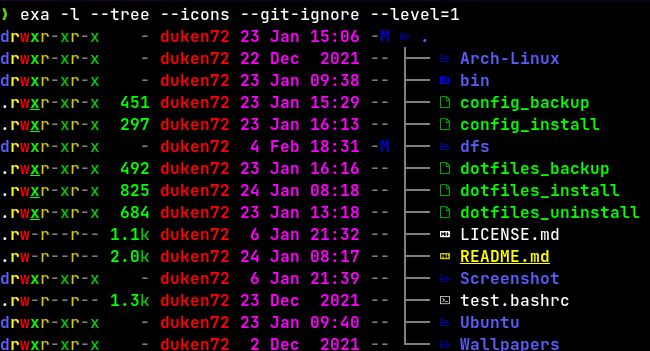
\includegraphics[width=0.9\textwidth]{exa.png}
		\caption{Viewing file system with \texttt{exa}.}
	\end{figure}

	\item View files or directories descriptions: \verb|file, du|, \verb|cloc| \cite{cloc}, \verb|tokei| \cite{tokei}
	
	\verb|file| - determine file type, \verb|du| - estimate file space usage, \verb|cloc| - count lines of code, \verb|tokei| - display statistics about your code. Some additional info regarding number of code lines, files, file and directory memory size, comments, \etc, is also needed. These info can be accessed and included with these commands. Example of \texttt{tokei}:
	\begin{verbatim}
	================================================================
	Language        Files    Lines     Code    Comments     Blanks
	================================================================
	BASH                8      118       85          14         19
	C Header           26     1871      986         528        357
	C++                16     3373     2627         326        420
	Makefile            2       60       38           4         18
	Python              1      173      110          36         27
	Shell               4     1669     1392         162        115
	Plain Text          4       98        0          86         12
	Zsh                14    20719    13838        5146       1735
	----------------------------------------------------------------
	Markdown            8     2998        0        2225        773
	|- BASH             3      119      103           6         10
	|- C++              1      137      132           0          5
	|- Lua              2        8        8           0          0
	|- YAML             2        6        6           0          0
	|- Zsh              3      167      136          20         11
	(Total)                   3435      385        2251        799
	================================================================
	Total              83    31079    19076        8527       3476
	================================================================
	\end{verbatim}
	
	\item Change ownership, permission: \verb|chown|, \verb|chmod|.
	
	\verb|chown| - change file or directory ownership, \verb|chmod| - change file or directory permissions.
	\item Search for file: \verb|locate, find|, \verb|fdfind| \cite{fdfind}, \verb|fzf| \cite{fzf}.
	
	\verb|locate| - list files in databases that match a pattern, \verb|find| - search for files in a directory hierarchy, \verb|fdfind| - user-friendly alternative to \texttt{find}, \verb|fzf| - a general-purpose command-line fuzzy finder.
	\begin{figure}[hbt!]
		\centering
		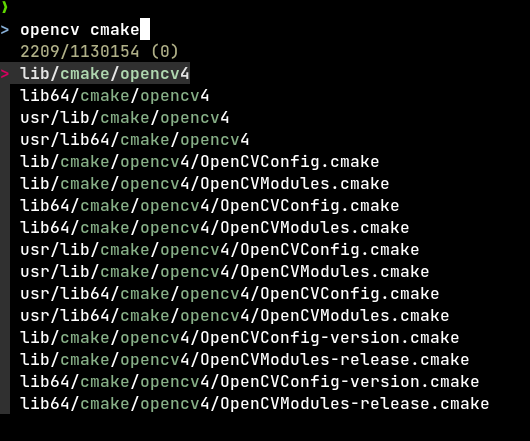
\includegraphics[width=0.9\textwidth]{fzf.png}
		\caption{Searching for file with fuzzy finder \texttt{fzf}.}
	\end{figure}
	\item Read guidance: \verb|man|, \verb|which|, \verb|apropos|, \verb|type|.
	
	\verb|man| - an interface to the system reference manuals, \verb|which| - shows the full path of (shell) commands, \verb|apropos| - search the manual page names and descriptions, \verb|type| - write a description of command type.
	
	\item Manage files and directories: \verb|mkdir|, \verb|rmdir|, \verb|touch|, \verb|cp|, \verb|mv|, \verb|rm|, \verb|ln|.
	
	\verb|mkdir| - make directories, \verb|rmdir| - remove empty directories, \verb|touch| - change file timestamps, \verb|cp| - copy files and directories, \verb|mv| - move (rename) files, \verb|rm| - remove files or directories, \verb|ln| - make links between files.
	
	\item View file content: \verb|cat, more, less|, \verb|bat| \cite{bat}.
	
	\verb|cat| - concatenate files and print on the standard output, \verb|more| - file filter for paging through text one screenful at a time, \verb|less| - provide \verb|more| emulation plus extensive enhancements, \verb|bat| - a \verb|cat| clone with syntax highlighting and Git integration.
	
	\item Edit file content: \verb|nano|, \verb|gedit|, \verb|vi|, \verb|vim|, \verb|sed|, \verb|sd| \cite{sd}, \verb|awk|, or file-specific application.
	
	Example commands for \texttt{sd} and \texttt{sed}:
	\begin{verbatim}
		sd [prev_expression] [new_expression] [file]
		sd [prev_expression] [new_expression] [file] -p #p-preview
		# just print out the results
		sed 's/[prev_expression]/[new_expression]/g' [file.txt]
		# replace a string with another
		sed -i 's/[prev_expression]/[new_expression]/g' [file.txt]
		sed '/searchStr/c\newLine' [file.txt] # replace a line contain a string
		
		awk '/pattern/ {print $2}' file.txt
		awk -f awkFD.awk file.txt
	\end{verbatim}
	
	\item Archive: \verb|zip|, \verb|unzip|, \verb|zipcloak|, \verb|zipslit|, \verb|tar|, \verb|gzip|, \verb|gunzip|, \verb|unrar|.
	
	\verb|zip| - package and compress (archive) files, \verb|unzip| - list, test and extract compressed file in a ZIP archive, \verb|zipcloak| - encrypt entries in a ZIP file, \verb|zipslit|, \verb|tar| - an archiving utility, \verb|gzip|, \verb|gunzip| - compress and expand files, \verb|unrar| - uncompress RAR archive .
	
	Some of the tags for \texttt{zip} are: \texttt{-r} for recursive search, \texttt{-e} for encryption, \texttt{-v} for more verbose output, \texttt{-9} for better compression. Example of recursive compression with encryption:
	\begin{verbatim}
		zip -er9 output.zip file1 file2
	\end{verbatim}
	Some tags for \texttt{unzip} are: \texttt{-x} for files exclusion, \texttt{-o} for overwrite, \texttt{-n} for not-overwrite, \texttt{-d} for output directory, \texttt{-l} for listing content. Examples of uncompress a \texttt{.zip} file:
	\begin{verbatim}
		unzip -o input.zip -x *.h -d target_dir
		upzip -l input.zip
	\end{verbatim}
	Additional commands for \texttt{.zip} files:
	\begin{verbatim}
		zipcloack file.zip # add password
		zipsplit -n [size_in_bytes] file.zip # split to size restriction
	\end{verbatim}
	Some tags for \texttt{tar}: \texttt{v} for more verbose output, \texttt{f} for files, \texttt{c} for create, \texttt{z} for \texttt{.gunzip} file, \texttt{x} for extract, \texttt{t} for listing. Examples of \texttt{tar} commands:	
	\begin{verbatim}
		tar cvf [target_file.tar] [files/dirs] # create .tar
		tar zcvf [target_file.tar.gz] [files/dirs] # create .tar.gz
		tar tvf [file.tar] # list out files in file.tar
		tar xvf [file.tar] -C [dirs] # extract tar file
		tar xvfz [file.tar.gz] [dirs] # extract tar.gz file
	\end{verbatim}
	
	Other commands with \verb|gzip, gunzip, unrar| for archiving and compression:
	\begin{verbatim}		
		gzip [file.tar] # compress the tar file to .tar.gz file
		gunzip [file.tar.gz] # uncompress the .tar.gz file to .tar file
		unrar x [file.rar]
	\end{verbatim}
	
	\item Monitor your system: \verb|htop|, \verb|neofetch|
	
	\texttt{htop} is the equivalent Linux-version of Task Manager in Windows, from which user can inspect current running process, application, in terms of memory, CPU percentages, end a process if desired.
	\begin{figure}[hbt!]
		\centering
		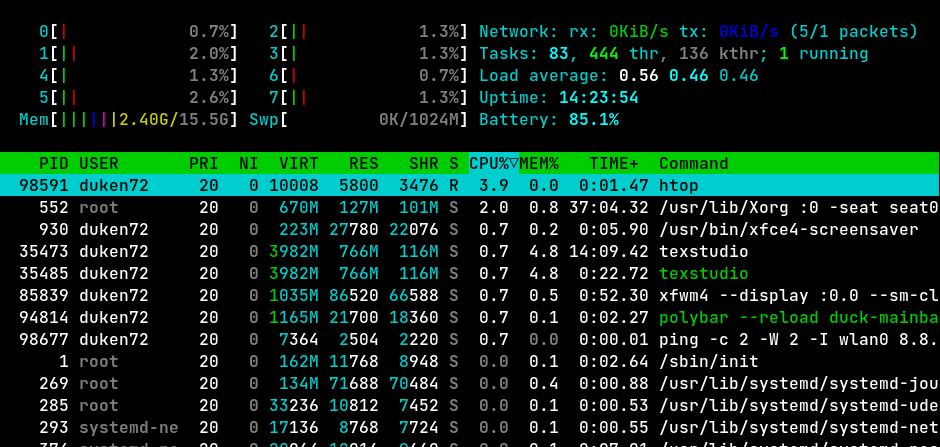
\includegraphics[width=0.9\textwidth]{htop.png}
		\caption{System inspection with \texttt{htop}.}
	\end{figure}
	\begin{figure}[hbt!]
		\centering
		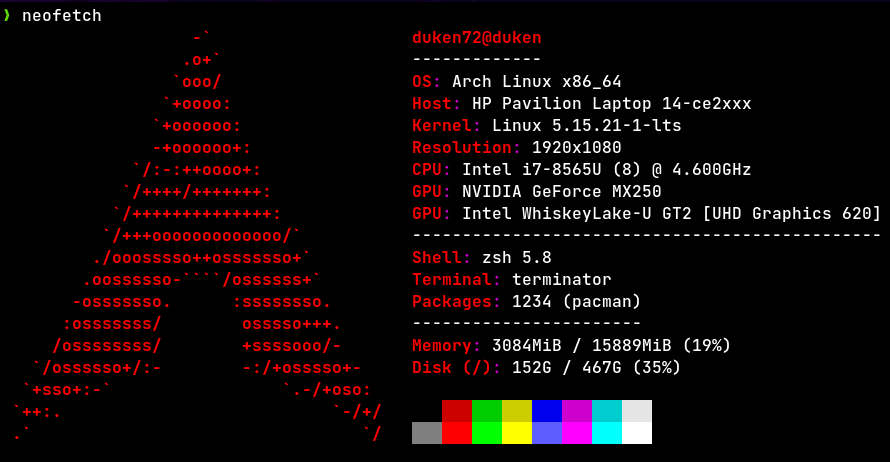
\includegraphics[width=0.9\textwidth]{neofetch.png}
		\caption{System inspection with \texttt{neofetch}.}
	\end{figure}

	\item Cryptography: \verb|openssl|
	
	Example commands:
	\begin{verbatim}
		openssl aes-256-cbc -salt -pbkdf2 -in <file.name> -out <file.enc.name>
		openssl aes-256-cbc -d -pbkdf2 -in <file.enc.name> -out <file.dec.name>
		cmp <file1> <file2> | echo \$? \#compare 2 file, 0 if same, 1 if different	
	\end{verbatim}
	\item Managing working processes: \verb|fg|, \verb|bg|, \verb|jobs|, \verb|kill|.
	
	\verb|fg| - run jobs in the foreground, \verb|bg| - run jobs in the background, \verb|jobs| - display status of jobs in the current session, \verb|kill| - terminate a process.	
\end{itemize}

\subsection{Shell scripting}

As a scripting language, user-defined aliases and programs could incorporate different basic commands. On top of a Shell program, the shebang must be included: \verb|#!/bin/sh| or \verb|#!/bin/bash|. The Shell language allows defining variables, accessing arguments, logical operator, flow control, etc.

\subsubsection{Variables to access}

The variables are accessed via \verb|$| sign.
\begin{itemize}
	\setlength\itemsep{0em}
	\item \verb|$0| - Name of the script
	\item \verb|$1| to \verb|$9| - Arguments to the script. \verb|$1| is the first argument and so on.
	\item \verb|$@| - All the arguments
	\item \verb|$#| - Number of arguments
	\item \verb|$?| - Return code of the previous command
	\item \verb|$$| - \ac{PID} for the current script
	\item \verb|!!| - Entire last command, including arguments, \eg: \verb|sudo !!| if last command fail due to permission
	\item \verb|$_| - Last argument from the last command.
\end{itemize}

\subsubsection{Logical operators}
There are three logical operators:
\begin{itemize}
	\setlength\itemsep{0em}
	\item The \texttt{||} operator:
	\begin{verbatim}
		false || echo "Oops, fail" # Oops, fail
		true || echo "Will not be printed"
	\end{verbatim}
	\item The \verb|&&| operator acts like an \texttt{AND} operator:
	\begin{verbatim}
		true && echo "Things went well" # Things went well
		false && echo "Will not be printed"		
	\end{verbatim}
	\item The \texttt{;} operator acts like an \texttt{OR} operator:
	\begin{verbatim}
		true ; echo "This will always run"
		false ; echo "This will always run"
	\end{verbatim}
\end{itemize}

\subsubsection{Flow controls}
With \ac{BASH}, there are flow controls just like in common languages, \eg, Python or C++.
\begin{itemize}
	\setlength\itemsep{0em}
	\item If-else statement:
	\begin{verbatim}
		if conditions; then
		  commands
		[elif conditions; then
		  commands]
		[else conditions; then
		  commands]
		fi
		
		# Multiple conditions:
		if ([condition1] || [condition2]) && [condition3]; then
		  commands
		fi
	\end{verbatim}
		
	\item For loop:
	\begin{verbatim}
		for i in word1 word2 word3; do
		  echo "$i"
		done
		
		for i in "$@"; do
		  echo $i
		done
	\end{verbatim}
	\item While loop:
	\begin{verbatim}
		while [ condition ] do
		  command1
		  command2
		  command3
		done
	\end{verbatim}
	
\end{itemize}

\subsubsection{Comments}
\begin{itemize}
	\setlength\itemsep{0em}
	\item Single line comments with "\verb|#|"\\
	Example: \verb|# Flow Control|
	\item Block comments
	\begin{verbatim}
	: <<'END'
	echo "I hope that there is no error"
	END
	\end{verbatim}
\end{itemize}

\subsubsection{Logic conditions}

Common logical conditions relate with file system. There are syntax to check whether a file exists and is of the expected type.

\begin{verbatim}
	if [ -d file ]; then echo "file is a directory" fi
	if [ -e file ]; then echo "file exists" fi
	if [ -f file ]; then echo "file exists and is a regular file" fi
	if [ -L file ]; then echo "file is a symbolic link" fi
	if [ -r file ]; then echo "file is a file readable by you" fi
	if [ -w file ]; then echo "file is a file writable by you" fi
	if [ -x file ]; then echo "file is a file executable by you" fi
	if type cmd; then echo "cmd exists" fi
	
	if [ file1 -nt file2 ]; then echo "file1 is newer than file2" fi
	if [ file1 -ot file2 ]; then echo "file1 is older than file2" fi
\end{verbatim}

In addition, there are syntax logic conditions to comparison between \texttt{string}:
\begin{verbatim}
	if [ -z string ]; then echo "string is empty" fi
	if [ -n string ]; then echo "string is not empty" fi
	if [ string1 = string2 ]; then echo "string1 equals string2" fi
	if [ string1 != string2 ]; then echo "string1 does not equal string2" fi
\end{verbatim}

\subsection{CLI Hotkeys}

It is useful to practice and remember some basic hotkeys while working on the \ac{CLI}. It should noted that different shells have different features regarding line completion and movements.

\begin{table}[hbt!]
	\centering
	\begin{tabular}{c|c}
		Commands   & Actions                           \\
		\hline\hline
		\verb|CTRL-A / E| & move to home/end of line       \\
		\verb|CTRL-F / B| & move for/backward a character   \\
		\verb|ALT -F / B| & move for/backward a word   \\
		\verb|CTRL-H| & delete char                  \\
		\verb|CTRL-W| & delete a word back             \\
		\verb|CTRL-K| & clear to end of line\\
		\verb|CTRL-U| & clear the line                   \\
		\verb|CTRL-S / Q| & toggle screen output       \\
		\verb|CTRL-L| & clear screen output            \\
		\verb|Ctrl-D| & exit shell                     \\
		\verb|CTRL-C| & stop current process          
	\end{tabular}
\end{table}

\section{CMake}

\subsection{Introduction}
CMake is a tool for build system, usually for projects or programs written in C or C++ language. Programmers write and work with source code. However, in order for the computers to understand and execute those programs, the source code needs to be built (compile and link with libraries) into binary file. Previously, \texttt{Makefile}s compile and build the source code, thus there is a need to maintain and update these \texttt{Makefile}s. As the project scale grows, this maintaining and updating tasks become more tedious. \Eg, when working with ROS, current package might use multiple external packages and libraries, which could have more than one executable, different build and test configurations. Build tools like CMake are developed to automate the complex build process. Instead of manually manage \texttt{Makefile}s, developers manage \texttt{CMakeLists.txt} file, which will create \texttt{Makefile}s. This section gives an overview on CMake.\\

\subsection{CMake Syntax}
CMake has its own scripting language, which includes variables, statements, flow control, commands, \etc. Some basic commands, syntax are as follows:
\begin{itemize}
	\setlength\itemsep{0em}
	\item Print message
	
	\verb|message("Hello world!")     # Print "Hello world!"|\\
	\verb|message("Hello ${NAME}!")   # Substitute a variable into the message|
	\item Assign variables
	
	\texttt{set(THING duck)}\\
	\verb|message("We want the ${THING}!")|
		
	In CMake, every variables are strings, which in most case relate to paths, names of files, libraries or configurations.
	\item Math operation
	
	\verb|math(EXPR MY_SUM "1 + 1")    # Store 2 in MY_SUM|\\
	\verb|message("The sum is ${MY_SUM}.")|	
	\item Flow control
	\begin{itemize}
		\item If-else statement
		\begin{verbatim}
			if(WIN32)
			  message("You're running CMake on Windows.")
			else()
			  message("You're not running CMake on Windows.")
			endif()
		\end{verbatim}
		\item While loop
		\begin{verbatim}
			set(A "1")
			set(B "1")
			while(A LESS "7")
			  message("A = ${A}")         # Print A
			  math(EXPR T "${A} + ${B}")  # Store the sum of A and B in T
			  set(A "${B}")               # Assign the value of B to A
			  set(B "${T}")               # Assign the value of T to B
			endwhile()
		\end{verbatim}
		\item For loop
		\begin{verbatim}
			foreach(ARG These are separate arguments)
			  message("${ARG}")       # Prints each word on a separate line
			endforeach()
		\end{verbatim}
		
	\end{itemize}	
	\item Combine commands with variable:
	\begin{verbatim}
		set(ARGS "EXPR;T;1 + 1")
		math(${ARGS})   # Equivalent to math(EXPR T "1 + 1")
		message("${ARGS}")
	\end{verbatim}
	\item List
	\begin{verbatim}
		set(MY_LIST These are separate arguments)
		message("${MY_LIST}")
		# Prints: These;are;separate;arguments
		
		set(MY_LIST These are separate arguments)
		list(REMOVE_ITEM MY_LIST "separate")
		# Removes "separate" from the list
		message("${MY_LIST}")
	\end{verbatim}
	\item Function
	\begin{verbatim}
		function(doubleIt VALUE)
		  math(EXPR RESULT "${VALUE} * 2")
		  message("${RESULT}")
		endfunction()
		
		# Prints: 8
		doubleIt("4")
	\end{verbatim}
	\item Marco
	\begin{verbatim}
		macro(doubleIt VARNAME VALUE)
		  # Set the named variable in caller's scope
		  math(EXPR ${VARNAME} "${VALUE} * 2")
		endmacro()
		
		# Tell the macro to set the variable named RESULT
		doubleIt(RESULT "4")					
		
		# Prints: 8
		message("${RESULT}")					
	\end{verbatim}
\end{itemize}

\subsection{CMake Target and Properties}
Targets are executable files, binary files. As the name itself suggests, they are the targets, the goal of CMake, to compile and build source code (in C++) to these executables. In other cases, instead of executable(s), the targets to build could be libraries, which are groups of functionalities that could be used somewhere else. The commands to define these targets are:
\begin{itemize}
	\setlength\itemsep{0em}
	\item \verb|add_executable|: define the target
	\item \verb|add_subdirectory, add_library, add_custom_target|: call \verb|CMakeLists.txt| from lower directory level.
\end{itemize}

These executables have properties, which are to be managed in order for the source code to be compiled and linked properly. Some common properties are:
\begin{itemize}
	\setlength\itemsep{0em}
	\item \verb|INCLUDE_DIRECTORIES|
	
	Include directories are where to find the C++ header files. With correct paths, header files can be included on top of the \verb|.cpp| files: \verb|#include <something.h>|. This is where the compiler will find function declarations, type definitions, classes, structures, \etc.
	\item \verb|LINK_LIBRARIES|
	
	While compiler concerns with the declarations, linker concerns with functions, methods definitions. These are handled by link libraries. In the build process, a target has to be compiled and linked in order to become a executable.
	\item \verb|COMPILE_DEFINITIONS|
	\item \verb|COMPILE_OPTIONS|
\end{itemize}

The commands to change or update these properties:

\begin{itemize}
	\setlength\itemsep{0em}
	\item \verb|(target_)include_directories|
	\item \verb|(target_)link_libraries|
	\item \verb|(target_)compile_definitions|
	\item \verb|(target_)compile_options|
	\item \verb|set_property|
	\item \verb|get_property|
\end{itemize}

For example, the following line gets the the \verb|SOURCES| property of the target \texttt{MyApp} and assigns it to \verb|MYAPP_SOURCES|:

\verb|get_property(MYAPP_SOURCES TARGET MyApp PROPERTY SOURCES)|

\subsection{Build Types}

There are different build types:
\begin{itemize}
	\setlength\itemsep{0em}
	\item \verb|Release|: high optimization level, no debug info, code or asserts.
	\item \verb|Debug|: No optimization, asserts enabled, custom debug (output) code enabled, debug info included in executable (so you can step through the code with a debugger and have address to source-file:line-number translation).
	\item \verb|RelWithDebInfo|: optimized, with debug info, but no debug (output) code or asserts.
	\item \verb|MinSizeRel|: same as Release but optimizing for size rather than speed.
\end{itemize}

In case of missing \verb|FindPackage.cmake| error, one could search for customized script online and put it in the package directory as follow:

\begin{figure}[hbt!]
	\centering
	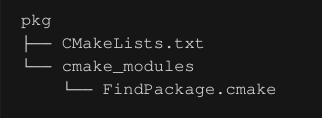
\includegraphics[width=0.7\textwidth]{findPackageCmake.png}
\end{figure}

In the top-level \verb|CMakeLists.txt|, add this line before \verb|find_package|:\\

\verb|list(APPEND CMAKE_MODULE_PATH ${CMAKE_CURRENT_LIST_DIR}/cmake_modules)|

\section{C++}
C++ is a statically typed programming language. On the other hand, Python is a dynamically typed programming language, which implies that developers don't have to think and define the type of all variables with care. C++ allows low-level memory and hardware control like the C language, but with high-level abstraction with classes and structures. With its computational and memory efficiency, the language has usage in game engines, databases, embedded systems, desktop software, \etc. When working with \ac{ROS}, the coding languages are C++ and Python. However, for most real-time operations and features, C++ is more preferable.

\subsection{Memory Management and Pointer}

\subsubsection{Variable types and sizes}

The primitive data types vary in the memory size that they occupy. Be aware that sometimes, the actual memory size also depends on the compiler or the data models. In addition, there are modifiers to the type:

\begin{itemize}
	\setlength\itemsep{0em}
	\item Signedness
	 \begin{itemize}
	 	\setlength\itemsep{0em}
		\item \verb|signed| (default) - have signed representation, loosing 1 bit
		\item \verb|unsigned| - have unsigned representation
	\end{itemize}
	\item Size \begin{itemize}
		\setlength\itemsep{0em}
		\item \verb|short| - be optimized for space and will have width of at least 16 bits.
		\item \verb|long| - have width of at least 32 bits.	
	\end{itemize}
\end{itemize}

\begin{table}[htb!]
	\centering
	\begin{tabular}{rcc}
		\textbf{Type}          & \textbf{Size}     & \textbf{Typical Range}   \\
		\hline\hline
		boolean                & 8 bits = 1 byte   & $0-1$                    \\
		(signed) char          & 8 bits = 1 byte   & $-2^7$ to $2^7-1$        \\
		unsigned char          & 8 bits = 1 byte   & $0$ to $2^8-1$           \\
		(signed) int           & 32 bits = 4 bytes & $-2^{31}$ to $2^{31}-1$  \\
		unsigned int           & 32 bits = 4 bytes & $0$ to $2^{32}-1$        \\
		(signed) short int     & 16 bits = 2 bytes & $-2^{15}$ to $2^{15}-1$  \\
		unsigned short int     & 16 bits = 2 bytes & $0$ to $2^{16}-1$        \\
		(signed) long int      & 32 bits = 4 bytes & $-2^{31}$ to $2^{31}-1$  \\
		unsigned long int      & 32 bits = 4 bytes & $0$ to $2^{32}-1$        \\
		(signed) long long int & 64 bits = 8 bytes & $-2^{63}$ to $2^{63}-1$  \\
		unsigned long long int & 64 bits = 8 bytes & $0$ to $2^{64}-1$        \\
		float                   & 32 bits = 4 bytes & $3.4E\pm38$ (7 digits)   \\
		double                 & 64 bits = 8 bytes & $1.7E\pm308$ (15 digits)
	\end{tabular}
	\caption{Data types with their size and range.}
\end{table}

A \verb|boolean| just needs 1 bit, but you can only access byte, thus it still occupies 1 byte, which is 8 bits. We could however store 8 \verb|bool|(s) in 1 byte. Suffixes are used to differentiate types when assigning variables. These suffixes are case-insensitive: \ie, `u` is equivalent to `U`, `UL` is equivalent to `uL, Ul, ul`.

\begin{table}[htb!]
	\centering
	\begin{tabular}{ccc}
		\textbf{Data Type} & \textbf{Suffix}   & \textbf{Meaning}   \\
		\hline\hline
		int                & U               & unsigned int       \\
		int                & L               & long               \\
		int                & UL / LU         & unsigned long      \\
		int                & LL              & long long          \\
		int                & ULL / LLU       & unsigned long long \\
		double             & F               & float               \\
		double             & L               & long double       
	\end{tabular}
	\caption{Suffixes for data types.}
\end{table}

\subsubsection{Stack and Heap Memory}

Allocating on the stack is fast, simple as only one CPU commands. There is a lot happen behind the scene when assigning a value on heap memory. To find the free space, assign, book keeping, .. In case you have something very memory heavy, then you have to use the heap.

\begin{itemize}
	\setlength\itemsep{0em}
	\item Allocate with the stack:\\
	\verb|int value = 5;|	
	\item Allocate with the heap:\\
	\verb|int* hvalue = new int;|\\
	\verb|*hvalue = 5;|
\end{itemize}

\subsubsection{new and delete operator}

The \verb|new| operator does two things: allocating memory and calling the constructor. The main purpose of \verb|new|, is to allocate memory, on the HEAP specifically. The \verb|delete| operator calls the destructor and then frees the memory.

Additional notes:
\begin{itemize}
	\setlength\itemsep{0em}
	\item Arrays created with \verb|new []| must be destroyed with \verb|delete[]|.
	\item Using \verb|new|, the object created remains in existence until you \verb|delete| it. Without using \verb|new|, the object will be destroyed when it goes out of scope.
	\item Every time you type \verb|new|, type \verb|delete|.
\end{itemize}

\subsubsection{Smart Pointers}

Unconscious not deallocating a pointer causes a memory leak that may lead to crash of the program. For languages with Garbage Collection Mechanisms to smartly deallocate unused memory, \eg, Java and C\#, programmers don't have to worry about memory leak. C++11 comes up with its own mechanism: Smart Pointer. When the object is destroyed, it frees the memory as well.

With \verb|#include <memory>|:
\begin{itemize}
	\setlength\itemsep{0em}
	\item \verb|std::unique_ptr| stores one pointer only. We can assign a different object by removing the current object from the pointer.
	\item \verb|std::shared_ptr| allows more than one pointer pointing to this one object at a time and it’ll maintain a Reference Counter using \verb|use_count()| method.
	\item \verb|std::weak_ptr| also allows more than one pointer pointing at one object at a time, but without a Reference Counter.
	\item \verb|std::auto_ptr| is replaced by \verb|std::unique_ptr|, with similar functionality, improved security, added features and support for arrays.
\end{itemize}

Good practice is to use \verb|std::make_shared| as a simple and more efficient way to create an object and a \verb|std::shared_ptr| to manage shared access to the object at the same time.

Let look into an example with these smart pointers. Assuming we have a \texttt{class A} with a simple method \texttt{show()}:
\begin{verbatim}
#include <memory>
#include <iostream>

class A
{
public:
  void show()
  {
    std::cout << "Run A::show()" << std::endl;
  }
};
\end{verbatim}

Initially, we can define also \verb|std::auto_ptr|. After C++11, this is depreciated.
\begin{verbatim}
int main()
{
  std::auto_ptr<A> p1(new A);
  p1->show();
  std::cout << "Memory address of p1 " << p1.get() << std::endl;
  std::auto_ptr<A> p2(p1);
  p2->show();
  std::cout << "Memory address of p1 " << p1.get() << std::endl;
  std::cout << p2.get() << std::endl;
}
\end{verbatim}

Example define and use \verb|std::unique_ptr|:
\begin{verbatim}
int main()
{
  std::unique_ptr<A> p1(new A);
  p1->show();
  std::cout << "Memory address of p1 " << p1.get() << std::endl;
}
\end{verbatim}

Since \verb|std::unique_ptr| allows only one pointer, attempt to copy will lead to error. The only way is to transfer the ownership
\begin{verbatim}
// Error: can't copy unique_ptr
// std::unique_ptr<A> p2 = p1;

// transfers ownership to p2
std::unique_ptr<A> p2 = move(p1);
p2->show();
std::cout << "Memory address of p1 " << p1.get() << std::endl;
std::cout << "Memory address of p2 " << p2.get() << std::endl;
std::cout << std::endl;
\end{verbatim}
Example create and use \verb|std::shared_ptr|

\begin{verbatim}
int main()
{
  std::cout << "smart_ptr example:" << std::endl;
  std::shared_ptr<A> p3(new A);
  std::cout << "Memory address of p3 " << p3.get() << std::endl;
  p3->show();
  std::shared_ptr<A> p4(p3);
  p4->show();
  std::cout << "Memory address of p3 " << p3.get() << std::endl;
  std::cout << "Memory address of p4 " << p4.get() << std::endl;  
  // Returns the number of shared_ptr objects
  // referring to the same managed object.
  std::cout << "Counts: " << p3.use_count() << std::endl;
  std::cout << "Counts: " << p4.use_count() << std::endl;
  // Relinquishes ownership of p1 on the object
  // and pointer becomes NULL
  p3.reset();
  std::cout << "Memory address of p3 " << p3.get() << std::endl;
  std::cout << "Counts: " << p4.use_count() << std::endl;
  std::cout << "Memory address of p4 " << p4.get() << std::endl;
  std::cout << std::endl;
}
\end{verbatim}

In practice, it is better to create this pointers with \verb|std::make_shared| or \verb|std::make_unique|
\begin{verbatim}
int main()
{
  // Good practice
  std::shared_ptr<A> p5 = std::make_shared<A>();
  std::unique_ptr<A> p5 = std::make_unique<A>();
}
\end{verbatim}

\subsection{Class Features}

\subsubsection{Constructor member initializer lists}

Normal constructor initialization:
\begin{verbatim}
Something::Something(int memIn1, double memIn2)
{
  mem1 = memIn1;
  mem2 = memIn2;
  mem3 = 'c';
};
\end{verbatim}


There are cases that initialization of data members inside constructor doesn’t work and Initializer List must be used: non-static constant data members, reference members, performance reasons, avoid unnecessary call to a default constructor, \etc. Initializing member values with initializer lists is better. The initializer list is inserted after the constructor parameters, after the ":" and separated by a ",".
\begin{verbatim}
Something::Something(int memIn1, double memIn2)
: mem1{memIn1}, mem2{memIn2}, mem3{'c'} {};
\end{verbatim}

\subsubsection{Structure versus Class}

Some features to differentiate between the use of structure and class in C++:

\textbf{Structure:}
\begin{itemize}
	\setlength\itemsep{0em}
	\item Default access specifier will be \verb|public|.
	\item The instance of the structure is known as "Structure variable".
	\item A \verb|struct| is a bundle of several related elements, which needed to be tied up together in a certain context. When a collection of \ac{POD} is needed.
\end{itemize}

\textbf{Class:}
\begin{itemize}
	\setlength\itemsep{0em}
	\item Default access specifier will be \verb|private|.
	\item The instance of the class is known as Object of the class.
	\item A \verb|class| can do things with its methods and members.
	\item Operators to work on new data type can be defined using special methods (over-loading operators).
	\item One class can be used as the basis for definition of another. If you use inheritance, don't use \verb|struct|, use \verb|class|.
	\item Declaration of a var of the new class type requires just the name of the class: \verb|classA varA;|, not: \verb|struct structA varA;|
\end{itemize}

\subsubsection{Virtual and Override Specifier}

These two concerns with Runtime Polymorphism. Without \verb|virtual|, you get early binding. With \verb|virtual|, you get late binding.

\begin{verbatim}
class Base
{
public:
  void Method1() { std::cout << "Base::Method1" << std::endl; }
  virtual void Method2() { std::cout << "Base::Method2" << std::endl; }
};

class Derived : public Base
{
public:
  void Method1() { std::cout << "Derived::Method1" << std::endl; }
  void Method2() { std::cout << "Derived::Method2" << std::endl; }
};

Base* basePtr = new Derived ();
//  Note - constructed as Derived, but pointer stored as Base*
basePtr->Method1();  //  Prints "Base::Method1"
basePtr->Method2();  //  Prints "Derived::Method2"
\end{verbatim}

In the above example, \texttt{Method1()} is defined without \texttt{virtual} specifier, thus, when we call \texttt{basePtr->Method1();}, the early binding calls the definition from the \texttt{Base} class. On the other hands, \texttt{Method2()} is defined in the \texttt{Base} class with \texttt{virtual} specifier, which implies late binding. Therefore, when \texttt{basePtr->Method2();} is called, the method of the \texttt{Derived} class is called.\\

When using \verb|virtual| functions, it is possible to make mistakes while declaring the member functions of the derived classes. Using the \verb|override| identifier prompts the compiler to display error messages when these mistakes are made.

\begin{verbatim}
class Base
{
public:
  virtual void Method2() { std::cout << "Base::Method2" << std::endl; }
};

class Derived : public Base
{
public:
  // override identifier will give Error for miss-typing Metod2
  void Metod2() { std::cout << "Derived::Method2" << std::endl; } override
};
\end{verbatim}

\subsection{Best practices and tips}

\subsubsection{Inline Specifier}

Inlining concerns with the overhead cost for switching time of small functions. When the \verb|inline| function is called, the whole code of the \verb|inline| function gets inserted or substituted. This substitution is performed by the C++ compiler at compile time. Inlining is only a request to the compiler, not a command. There are cases that the compiler can ignore this request. \verb|inline| functions have advantages but also disadvantages.
\begin{verbatim}
inline int cube(int s)
{
  return s*s*s;
}
\end{verbatim}

For Class definition, you only need to add \verb|inline| when defining it, not when declaring it inside the class.

\subsubsection{Explicit Specifier}

Specifies that a constructor or conversion function (since C++11) or deduction guide (since C++17) is \verb|explicit|, that is, it cannot be used for implicit conversions and copy-initialization. Example of implicit specifier:
\begin{verbatim}
class A
{
public:
  A();
  A(int);
  A(const char*, int = 0);
};

int main()
{
  A c = 1;
  A d = "Venditti";
}
\end{verbatim}

In this example, though variable \texttt{c} is of \texttt{class A}, which is not an \texttt{int}, it is okay to write initialize \texttt{A c = 1;} due to implicit conversion. The same happens with \texttt{A d = "Venditti";}. The above program exits without error.\\

However, the above usage might lead to accidental construction that can hide bugs. Thus, we might want to turn off the implicit conversion with \texttt{explicit} specifier. Example of explicit specifier:
\begin{verbatim}
class A
{
public:
  explicit A();
  explicit A(int);
  explicit A(const char*, int = 0);
};

int main()
{
  A a2 = A(1);
  A a3(1);
  A a4 = A("Venditti");
  A a5 = (A)1;
  A a6 = static_cast<A>(1);
  return 0;
}
\end{verbatim}

\subsubsection{Keyword auto}

Use \verb|auto| to increase readability without creating confusion.
\begin{verbatim}
	// good : auto increases readability here
	// v could be array as well
	for(auto it = std::begin(v); it != std::end(v); ++it) {}
	
	// No type confusion
	auto obj1 = new SomeType<OtherType>::SomeOtherType();
	auto obj2 = std::make_shared<XyzType>(args...);
\end{verbatim}

\subsubsection{Using and Typedef Keywords}

Purposes of keyword \verb|using| in C++:

\begin{itemize}
	\setlength\itemsep{0em}
	\item \verb|using| declarations: brings a specific member from the \verb|namespace| into the current scope.
	\begin{verbatim}
		int main()
		{
		  using std::cout; // declare cout resolve to std::cout
		  cout << "Hello world!"; // no std:: prefix is needed here
		  return 0;
		} // the using declaration expires here
	\end{verbatim}
	\item \verb|using| directive: brings all members from a \verb|namespace| into the current scope.
	
	\verb|using namespace std;|
	
	In modern C++, \verb|using| directives generally offer little benefit (saving some typing) compared to the risk. Because \verb|using| directives import all of the names from a \verb|namespace| (potentially including lots of names you’ll never use), the possibility for naming collisions to occur increases significantly (especially if you import the \verb|std namespace|).
	\item Bring a base class method or variable into the current class’s scope.
	\item In C++11, the keyword \verb|using| is used for \verb|type alias|, which is identical to \verb|typedef|. In many cases, using has improving readability, compared to the equivalent \verb|typedef|, especially with pointer and template.
\end{itemize}

\section{VSCode}

VSCode is a code editor made by Microsoft. It is the most popular Development Environment (2019) \cite{devSurvey2019} with many features including support for debugging, syntax highlighting, code completion, snippets, refactoring, Git status, \etc. Visual Studio Marketplace \cite{vscode_marketplace} offers extensions for numerous coding languages, file types, integration with other tools and platforms, \etc.\\

\subsection{Hotkeys}

Some helpful VSCode hotkeys:
\begin{center}
\begin{tabular}{|l|l|}
	\hline	
	Command	& Action \\ [0.5ex] \hline\hline
	Ctrl + P & Find files \\
	Ctrl + Shift + E & File Explorers \\
	Ctrl + Shift + P & Show all commands \\
	Ctrl + Space & Invoke IntelliSense suggestion \\
	Ctrl + C (without text selection) & Copy entire current line \\
	Ctrl + Shift + K & Delete the entire line                      \\
	Alt + Move Arrow & Move entire selected line(s) up/down       \\
	Ctrl + F & Find words in file                                \\
	Ctrl + H & Find and replace words in file                    \\
	Ctrl + Shift + F & Find words in workspace                     \\
	Ctrl + Shift + H & Find and replace words in workspace         \\
	F2 & Rename Refactoring                                    \\
	F8 & Errors and Warning                                    \\
	Ctrl + Shift+I & Formatting                                   \\
	Ctrl + Shift+[ or ] & Code folding                           \\
	Ctrl + ` & Open Terminal                                   \\
	Ctrl + Shift+M & Open Problems                               \\
	Ctrl + Shift+X & Extensions                                  \\
	Ctrl + Shift+G & Git                                         \\
	Ctrl + , & Settings                                          \\
	Ctrl + . & Code actions                                      \\
	Ctrl + B & Close side panels                                 \\
	Ctrl + J & Code bottom panels                                \\
	Ctrl + \ & Split editor                                      \\
	Ctrl + 2 & Extra tab \\ [1ex] \hline
\end{tabular}
\end{center}

\subsection{Snippet}

Example of VSCode snippet:
\begin{verbatim}
"Snippet purpose": {
	 "prefix": "prefix_name",
	 "description": "Do something",
	 "body": [
	    "line 1",
	    "line 2",
	    "",
	    "line 3",
	    ""
	 ]
}
\end{verbatim}

\section{VIM}

Vim \cite{vim} is a free and open-source text editor for Unix. It is the abbreviation of Vi IMproved, which implies it is an improved clone of vi. It's a tool designed for coder. It has the capabilities to program commands.

\subsection{Modes}

There are three modes, and their corresponding keyboard to enter:

\begin{itemize}
	\setlength\itemsep{0em}
	\item \verb|ESC| - Command mode
	\item \verb|i| - Insert mode
	\item \verb|r| - Replace mode
	\item \verb|v| - Visual mode
\end{itemize}

\subsection{Basic commands}

Commands to save and exit:
\begin{itemize}
	\setlength\itemsep{0em}
	\item \verb|:q| - close a window, check vim window
	\item \verb|:qa| - quit all window
	\item \verb|:q!| - quit without writing
	\item \verb|:w| - write
	\item \verb|:wq| - save and exit
\end{itemize}

Commands for navigation:
\begin{itemize}
	\setlength\itemsep{0em}
	\item \verb|hjkl| - simple movement
	\item \verb|wbe| - words: next, beginning, end of word
	\item \verb|WBE| - words, but seperated by space
	\item \verb|Shift-HML| - screen top, middle, bottom
	\item \verb|Ctrl-UD| - scroll up/down
	\item \verb|Ctrl-G| - tell where you are
	\item \verb|Ctrl-FB| - scroll faster up/down
	\item \verb|f[char]| - find char in that line
	\item \verb|t[char]| - to char in that line. right before that char
	\item \verb|G| - move to bottom of the file
	\item \verb|gg| - move to start of the file
	\item \verb|:number| - go to line number	
\end{itemize}

Commands for editing:
\begin{itemize}
	\setlength\itemsep{0em}
	\item \verb|i| - insert mode
	\item \verb|r| - replace mode, then enter insert mode
	\item \verb|s| - \texttt{xi}, delete char, then enter insert mode
	\item \verb|d{motion}| - delete motion, \eg: \texttt{dw, de, dd, d\$, d0}
	\item \verb|c{motion}| - change motion, \eg: \texttt{cw, ce, cc, c\$, c0}
	\item \verb|y{motion}| - copy motion, \eg: \texttt{yw, yy, y\$, y0}
	\item \verb|D| - delete the remaining of line, equivalent with \texttt{d\$}
	\item \verb|C| - change the remaining of line, equivalent with \texttt{c\$}
	\item \verb|A| - append text at the end of line
	\item \verb|x / X| - delete/backspace character
	\item \verb|o / O| - insert line below/above and enter insert mode
	\item \verb|p / P| - paste after/before the cursor
	\item \verb|u| - undo last command
	\item \verb|U| - undo all commands in the current line
	\item \verb|Ctrl-r| - redo command
	\item \verb|.| - repeat the last command, could be somewhere else
	\item \verb|q<char>| - start record keystrokes into register \texttt{<char>}
	\item \verb|q| - stop record
	\item \verb|@<char>| - play recorded keystrokes into register \texttt{<char>}
	\item \verb|@@| - repeat last recording
	\item \verb|ci(| - change inside "(" bracket
	\item \verb|da{| - delete around "\{" bracket, so include "\{" and "\}"
\end{itemize}

Commands to replace:
\begin{itemize}
	\setlength\itemsep{0em}
	\item \verb|:s/str_1/str_2/| - replace first \texttt{str\_1} with \texttt{str\_2} in current line
	\item \verb|:s/str_1/str_2/g| - replace all \texttt{str\_1} with \texttt{str\_2} in current line
	\item \verb|:%s/str_1/str_2/g| - replace all \texttt{str\_1} with \texttt{str\_2} in whole file
	\item \verb|:2,7s/str_1/str_2/g| - replace all \texttt{str\_1} with \texttt{str\_2} in lines \texttt{2-7}
\end{itemize}

Commands to search:
\begin{itemize}
	\setlength\itemsep{0em}
	\item \verb|/[word]+Enter| - search for \texttt{word}
	\item \verb|n / shift-N| - go to next or previous searched \texttt{word}
\end{itemize}

Commands in Visual modes:
\begin{itemize}
	\setlength\itemsep{0em}
	\item \verb|v| - visual mode
	\item \verb|Shift-v| - visual line mode
	\item \verb|Ctrl-v| - visual block mode
\end{itemize}

Commands with counts:
\begin{itemize}
	\setlength\itemsep{0em}
	\item \verb|3w| - 3 words forward
	\item \verb|5j| - 5 lines down
	\item \verb|7dw| - delete 7 words
\end{itemize}

Commands with synced Vim window:
\begin{itemize}
	\setlength\itemsep{0em}
	\item \verb|Ctrl+w, s| - split horizontal
	\item \verb|:vsp| - split vertical
	\item \verb|Ctrl+w, v| - split vertical
	\item \verb|Ctrl+w, q| - close split window
	\item \verb|Ctrl+w, w| - switch around window
	\item \verb|Ctrl+w, hjkl| - switch around adjacent window
\end{itemize}

\clearpage